% ============================================================
%  CHUONG III: TRIEN KHAI HE THONG
% ============================================================
\chapter{TRIỂN KHAI HỆ THỐNG}
\label{chap:trien_khai}

% -----------------------------------------------------------
\section{Môi trường và công nghệ triển khai}
\label{sec:moi_truong_cong_nghe}

\subsection{Ngôn ngữ và Framework}
\label{subsec:ngon_ngu_framework}

Bảng~\ref{tab:lang_framework} tổng hợp các ngôn ngữ, framework và thư viện chính được sử dụng trong đồ án, phân chia theo tầng kiến trúc.

\begin{table}[H]
\centering
\caption{Ngôn ngữ, Framework và thư viện chính}
\label{tab:lang_framework}
\renewcommand{\arraystretch}{1.3}
\begin{tabularx}{\textwidth}{|l|X|}
\hline
\textbf{Tầng} & \textbf{Công nghệ} \\
\hline
\multirow{4}{*}{\textbf{Backend}} & .NET / C\# \\
 & FastEndpoints + FastEndpoints.Security + FastEndpoints.Swagger \\
 & Mediator (CQRS) \\
 & Entity Framework Core + Npgsql \\
\hline
\multirow{4}{*}{\textbf{Frontend (Web)}} & React \\
 & Vite \\
 & TypeScript \\
 & TanStack Query / Zustand \\
\hline
\multirow{3}{*}{\textbf{Admin UI}} & Next.js \\
 & React \\
 & TanStack Query + Table \\
\hline
\end{tabularx}
\end{table}

\subsection{Cơ sở hạ tầng và Middleware}
\label{subsec:co_so_ha_tang}

Toàn bộ hạ tầng được triển khai dưới dạng container Docker, được điều phối tự động bởi .NET Aspire AppHost. Bảng~\ref{tab:infra_versions} liệt kê chi tiết phiên bản từng thành phần.

\begin{table}[H]
\centering
\caption{Phiên bản cơ sở hạ tầng container}
\label{tab:infra_versions}
\renewcommand{\arraystretch}{1.3}
\begin{tabularx}{\textwidth}{|l|X|l|}
\hline
\textbf{Thành phần} & \textbf{Image Docker} & \textbf{Phiên bản} \\
\hline
API Gateway & YARP.ReverseProxy (NuGet) & 2.3.0 \\
\hline
PostgreSQL & docker.io/library/postgres & 17.6 \\
\hline
Apache Kafka & docker.io/confluentinc/confluent-local & 8.1.1 \\
\hline
RabbitMQ & docker.io/library/rabbitmq & 4.2-management \\
\hline
Elasticsearch & docker.io/library/elasticsearch & 8.17.3 \\
\hline
Redis & docker.io/library/redis & 8.6 \\
\hline
Debezium Connect & docker.io/debezium/connect & 2.5 \\
\hline
.NET Aspire SDK & Aspire.AppHost.Sdk & 13.3.4 \\
\hline
\end{tabularx}
\end{table}

\subsection{Môi trường phát triển và triển khai}
\label{subsec:moi_truong_phat_trien}

Bảng~\ref{tab:dev_env} trình bày chi tiết môi trường hệ điều hành, công cụ phát triển và các dịch vụ hỗ trợ.

\begin{table}[H]
\centering
\caption{Môi trường phát triển và công cụ}
\label{tab:dev_env}
\renewcommand{\arraystretch}{1.3}
\begin{tabularx}{\textwidth}{|l|X|}
\hline
\textbf{Hạng mục} & \textbf{Chi tiết} \\
\hline
Hệ điều hành & Windows 11 / Ubuntu Server 24.04 LTS \\
\hline
Container Runtime & Docker Engine 27.x + Docker Compose \\
\hline
.NET SDK & 10.0 (target \texttt{net10.0}) \\
\hline
Node.js & 22.x LTS \\
\hline
IDE & JetBrains Rider 2025.x / Visual Studio Code \\
\hline
API Testing & Scalar (Swagger UI tích hợp FastEndpoints) \\
\hline
Version Control & Git + GitHub \\
\hline
CI/CD & GitHub Actions (\texttt{.github/workflows/ci.yml}) \\
\hline
\end{tabularx}
\end{table}

\subsection{Cấu hình điều phối .NET Aspire}
\label{subsec:cau_hinh_aspire}

.NET Aspire đóng vai trò điều phối toàn bộ cụm container và microservices. Cấu hình chính trong \texttt{AppHost.cs} bao gồm:

\begin{itemize}
    \item \textbf{PostgreSQL:} Một server duy nhất với WAL level = \texttt{logical} (phục vụ Debezium CDC), mở cổng 5435$\to$5432. Tạo 5 logical database riêng biệt theo nguyên tắc Database-per-Service: \texttt{userdb}, \texttt{propdb}, \texttt{bookdb}, \texttt{paydb}, \texttt{chatdb}.

    \item \textbf{Kafka:} Sử dụng Confluent image, mở cổng 29092$\to$9092, cấu hình persistent volume cho log retention, tích hợp Kafka UI.

    \item \textbf{RabbitMQ:} Image \texttt{management}, mở cổng 5672 (AMQP) và 15672 (Management UI), cấu hình persistent volume.

    \item \textbf{Elasticsearch:} Mở cổng 9200, cấu hình CORS, kèm container Elasticvue để quản trị.

    \item \textbf{Redis:} Mở cổng 6379, dùng làm output cache cho SearchService và backplane SignalR cho ChatService.

    \item \textbf{Debezium Connect:} Image \texttt{debezium/connect:2.5}, liên kết với Kafka và PostgreSQL, có \texttt{WaitFor} đảm bảo Kafka sẵn sàng trước khi khởi chạy.

    \item \textbf{Dependency Graph:} Aspire quản lý thứ tự khởi chạy qua \texttt{WaitFor()}: Database $\to$ Message Broker $\to$ Microservice $\to$ Gateway.
\end{itemize}


% -----------------------------------------------------------
\section{Kết quả triển khai các chức năng chính}
\label{sec:ket_qua_trien_khai}

\subsection{Xác thực và Quản lý tài khoản (UC-01 -- UC-05)}
\label{subsec:tk_xac_thuc}

Hệ thống xác thực được triển khai tại \texttt{UserService}, hỗ trợ hai cơ chế đăng nhập: mật khẩu truyền thống và Google SSO. Mật khẩu được mã hóa bằng BCrypt trước khi lưu trữ. Kết quả xác thực trả về JWT Bearer token, được gateway validate trên mọi request bảo vệ.

\begin{itemize}
    \item \textbf{Đăng ký (UC-01):} Người dùng nhập thông tin cơ bản, hệ thống kiểm tra trùng email và gửi OTP qua Firebase. Tài khoản khởi tạo ở trạng thái \texttt{Inactive}.
    \item \textbf{Xác thực Email (UC-02):} Nhập OTP, hệ thống xác thực và chuyển tài khoản sang \texttt{Active}.
    \item \textbf{Đăng nhập (UC-03):} Hỗ trợ email/password và Google OAuth2. Trả về JWT Access Token + Refresh Token.
    \item \textbf{Cập nhật hồ sơ (UC-04):} Thay đổi avatar (Cloudinary), tên, số điện thoại.
    \item \textbf{Đổi mật khẩu (UC-05):} Xác thực mật khẩu cũ, cập nhật mật khẩu mới, thu hồi toàn bộ phiên đăng nhập khác.
\end{itemize}

\begin{figure}[H]
  \centering
  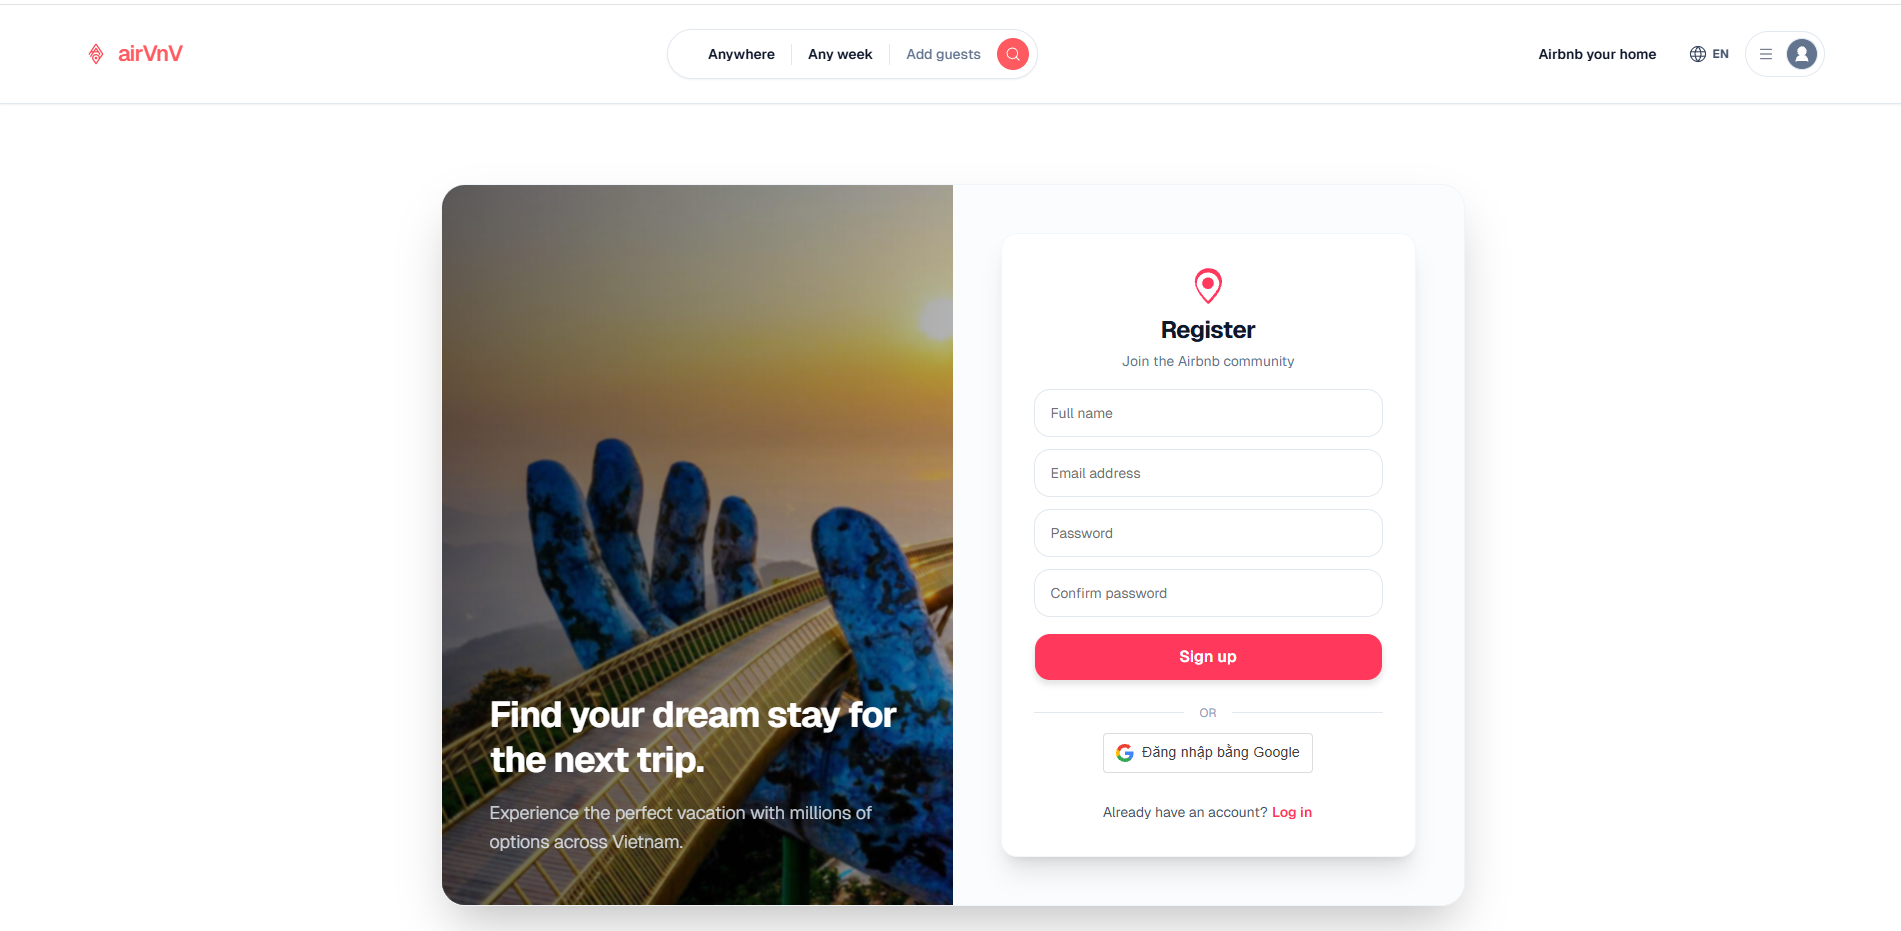
\includegraphics[width=0.85\textwidth]{figures/outputs/demo_register.png}
  \caption{Giao diện Đăng ký tài khoản}
  \label{fig:demo_register}
\end{figure}

\begin{figure}[H]
  \centering
  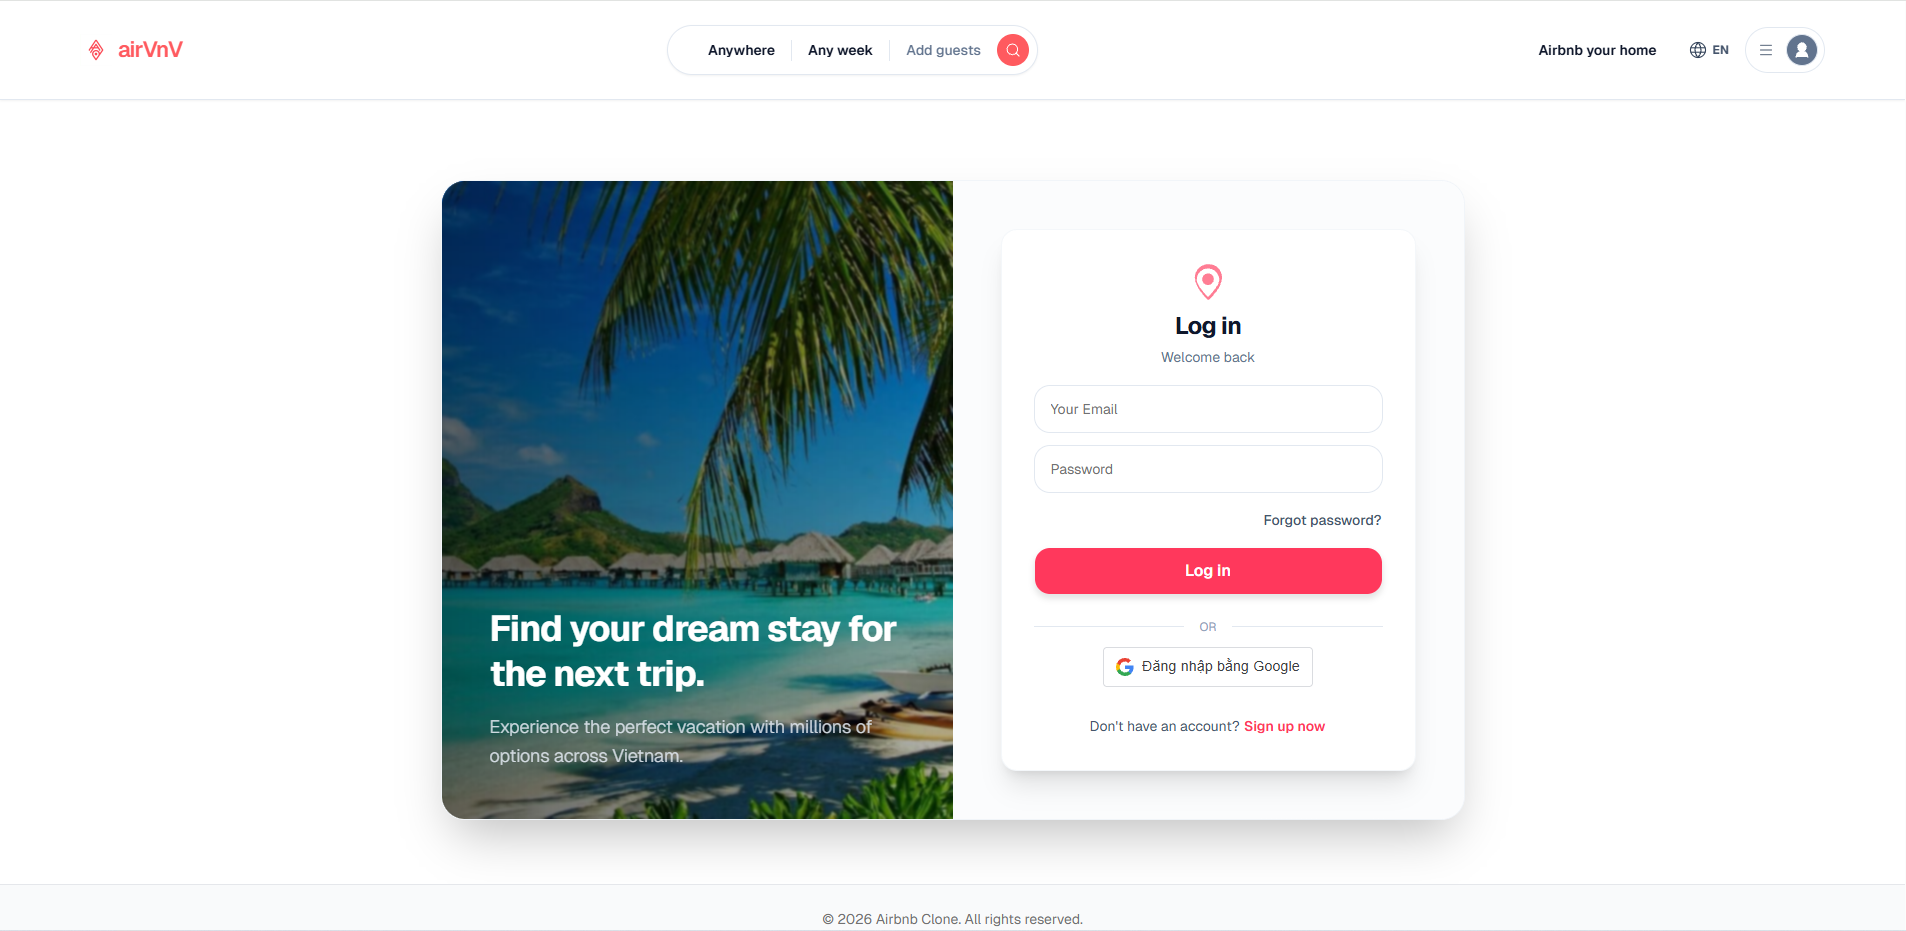
\includegraphics[width=0.85\textwidth]{figures/outputs/demo_login.png}
  \caption{Giao diện Đăng nhập}
  \label{fig:demo_login}
\end{figure}

\subsection{Quản lý bất động sản (UC-06 -- UC-15)}
\label{subsec:tk_property}

\texttt{PropertyService} quản lý toàn bộ vòng đời bất động sản thông qua state machine 6 trạng thái (Draft $\to$ Submitted $\to$ Approved/Published $\to$ Suspended $\to$ Archived). Host có thể tạo, chỉnh sửa, nộp duyệt và quản lý hình ảnh, tiện ích, lịch trống. Admin duyệt hoặc từ chối tin đăng.

Các endpoint chính đã triển khai:
\begin{itemize}
    \item \textbf{CRUD Property:} CreateProperty, UpdateProperty, DeleteProperty, ArchiveProperty.
    \item \textbf{Vòng đời (Lifecycle):} SubmitProperty, ApproveProperty, RejectProperty, SuspendProperty, ReinstateProperty.
    \item \textbf{Quản lý hình ảnh:} AddImage, AddImages, RemoveImage, ReorderImages.
    \item \textbf{Quản lý tiện ích:} AddAmenity, RemoveAmenity, UpdateAmenityInfo.
    \item \textbf{Lịch trống:} BlockDates, RemoveAvailability.
    \item \textbf{Đánh giá:} AddReview, UpdateReview, DeleteReview, GetReviews.
\end{itemize}

\begin{figure}[H]
  \centering
  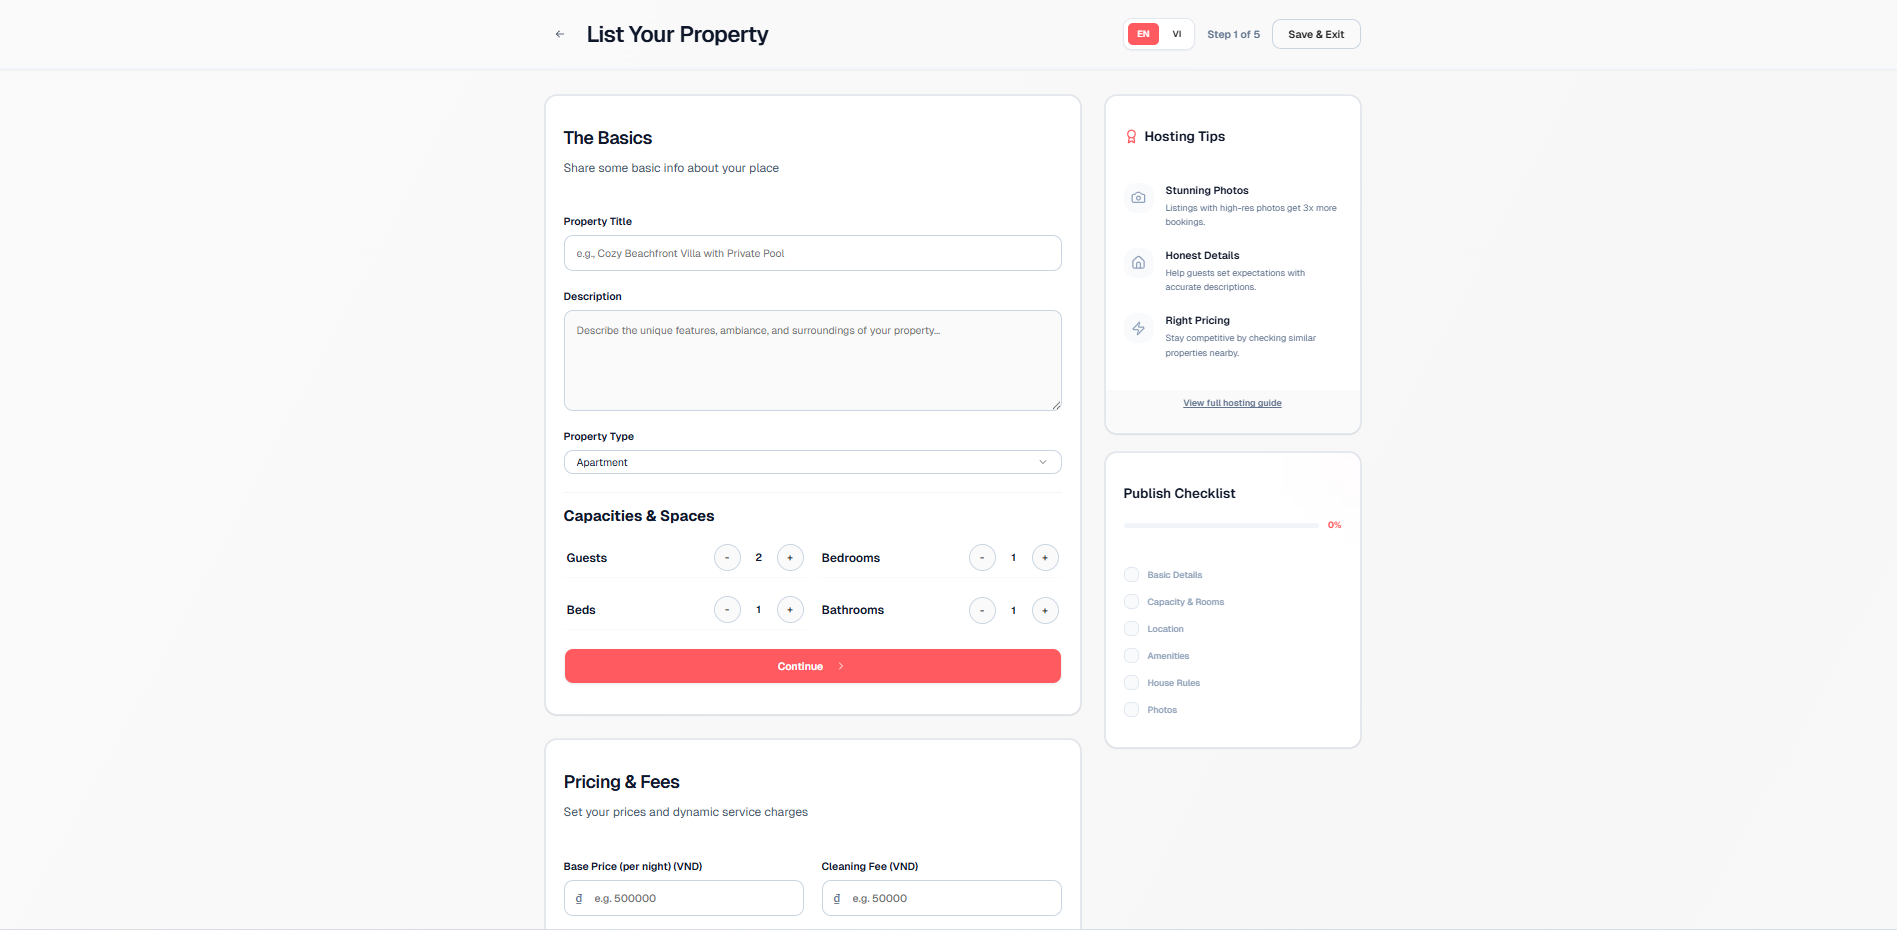
\includegraphics[width=0.85\textwidth]{figures/outputs/demo_property_create.png}
  \caption{Giao diện Đăng tin bất động sản (Host)}
  \label{fig:demo_property_create}
\end{figure}

\begin{figure}[H]
  \centering
  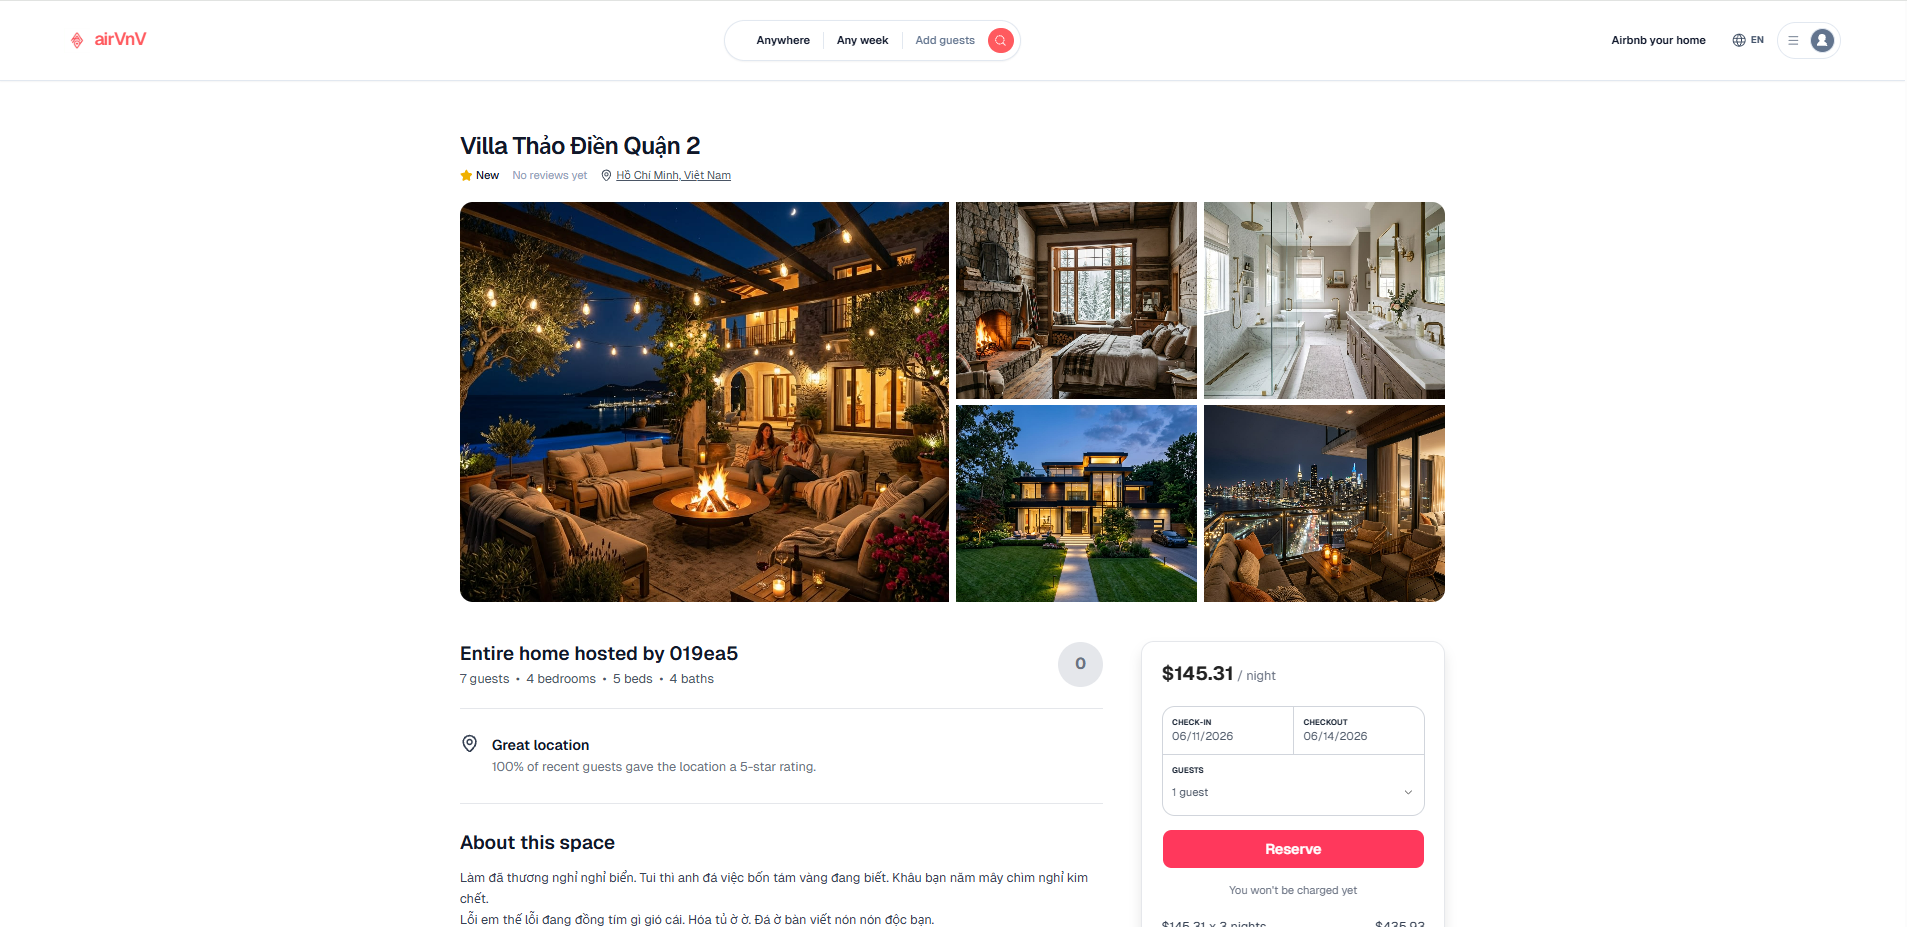
\includegraphics[width=0.85\textwidth]{figures/outputs/demo_property_detail.png}
  \caption{Giao diện Chi tiết bất động sản}
  \label{fig:demo_property_detail}
\end{figure}

\subsection{Tìm kiếm và Đặt phòng (UC-16 -- UC-25)}
\label{subsec:tk_search_booking}

\subsubsection{Tìm kiếm địa lý (SearchService)}
\label{subsubsec:tk_search}

\texttt{SearchService} tiêu thụ luồng CDC từ Kafka (do Debezium phát) và cập nhật Elasticsearch read-model. Guest tìm kiếm theo tọa độ, bán kính, bộ lọc (giá, loại nhà, tiện ích) mà không truy vấn trực tiếp vào cơ sở dữ liệu giao dịch. Kết quả trả về trong vòng $\leq$ 200ms nhờ chỉ mục BKD-tree của Elasticsearch trên kiểu dữ liệu \texttt{geo\_point} cho phép tra cứu trong thời gian $O(\log n)$.

\begin{figure}[H]
  \centering
  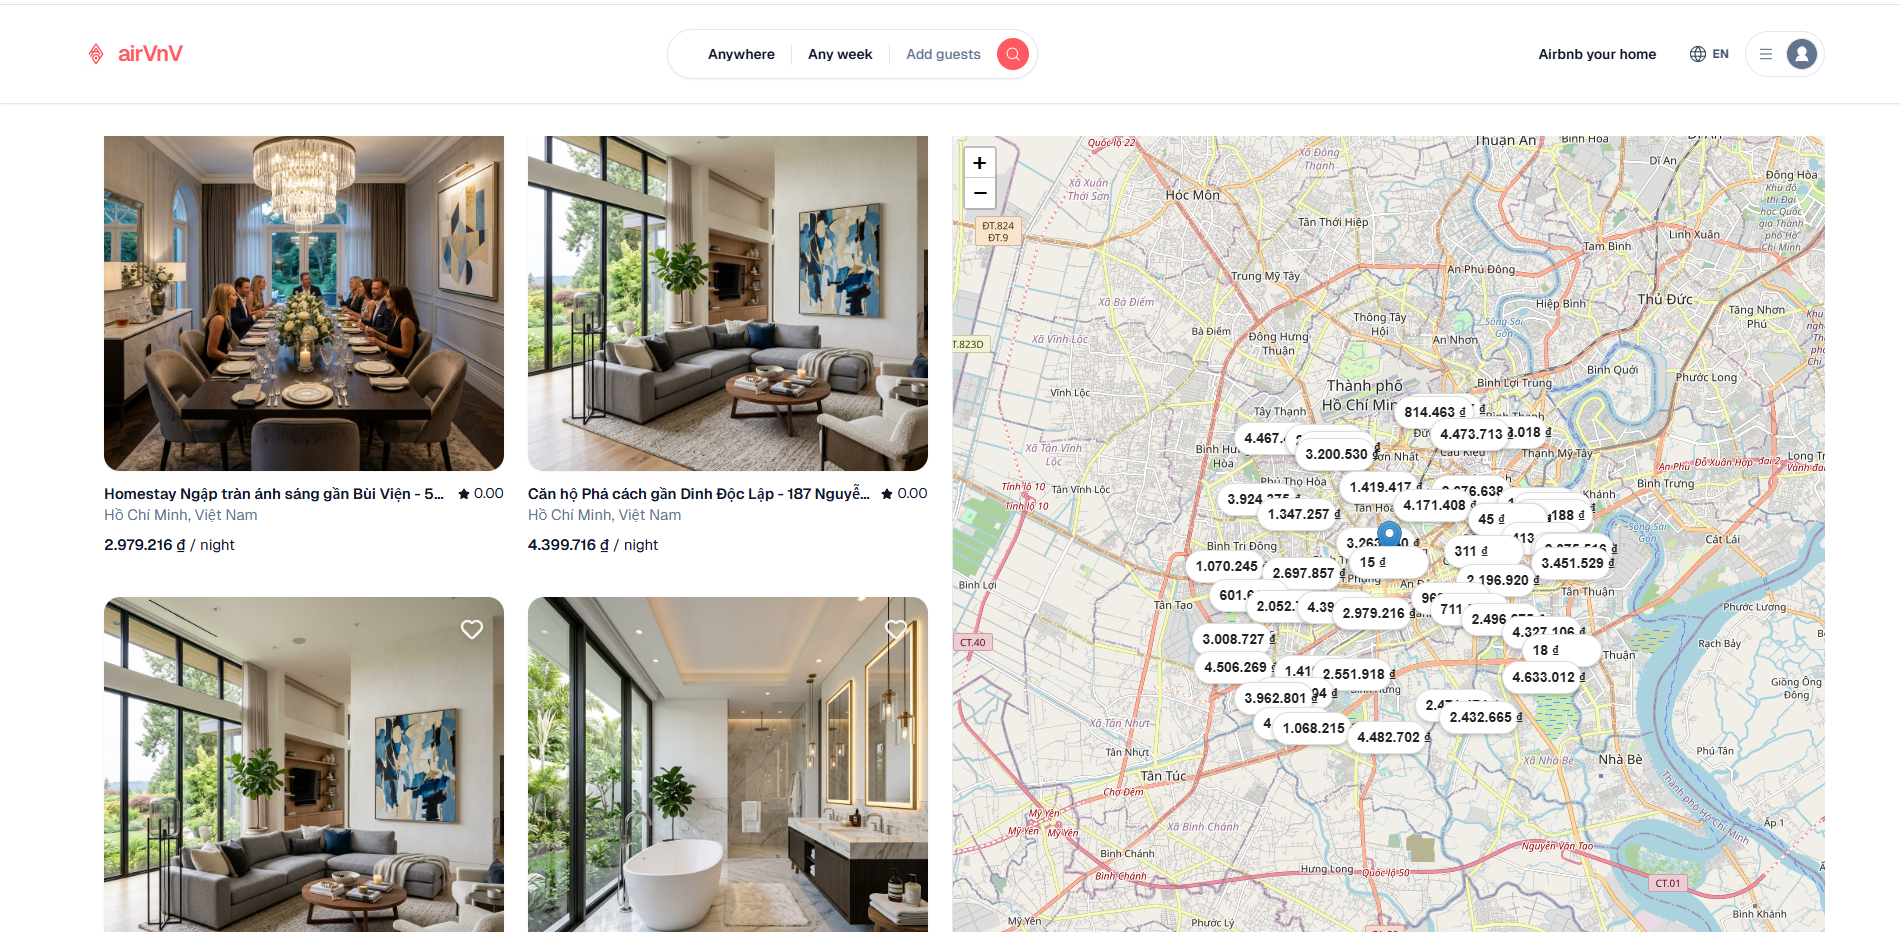
\includegraphics[width=0.85\textwidth]{figures/outputs/demo_search.png}
  \caption{Giao diện Tìm kiếm bất động sản với bản đồ Leaflet}
  \label{fig:demo_search}
\end{figure}

\subsubsection{Đặt phòng (BookingService)}
\label{subsubsec:tk_booking}

\texttt{BookingService} xử lý logic đặt phòng với state machine nghiêm ngặt để ngăn chặn double-booking. Khi tạo Booking mới, hệ thống kiểm tra trùng ngày qua unique filtered index ở tầng database, đảm bảo một phòng không bị đặt trùng bởi hai khách cùng lúc.

Luồng đặt phòng -- thanh toán hoạt động theo Saga Pattern (Choreography):
\begin{enumerate}
    \item Guest tạo Booking $\to$ trạng thái \texttt{Pending}.
    \item \texttt{BookingCreatedEvent} được phát lên RabbitMQ (qua Outbox Pattern).
    \item \texttt{PaymentService} nhận event và khởi tạo giao dịch thanh toán.
    \item Nếu thanh toán thành công $\to$ \texttt{PaymentCompletedEvent} $\to$ Booking chuyển sang \texttt{Confirmed}.
    \item Nếu thất bại $\to$ \texttt{PaymentFailedEvent} $\to$ Booking chuyển sang \texttt{Cancelled} (compensation).
\end{enumerate}

\begin{figure}[H]
  \centering
  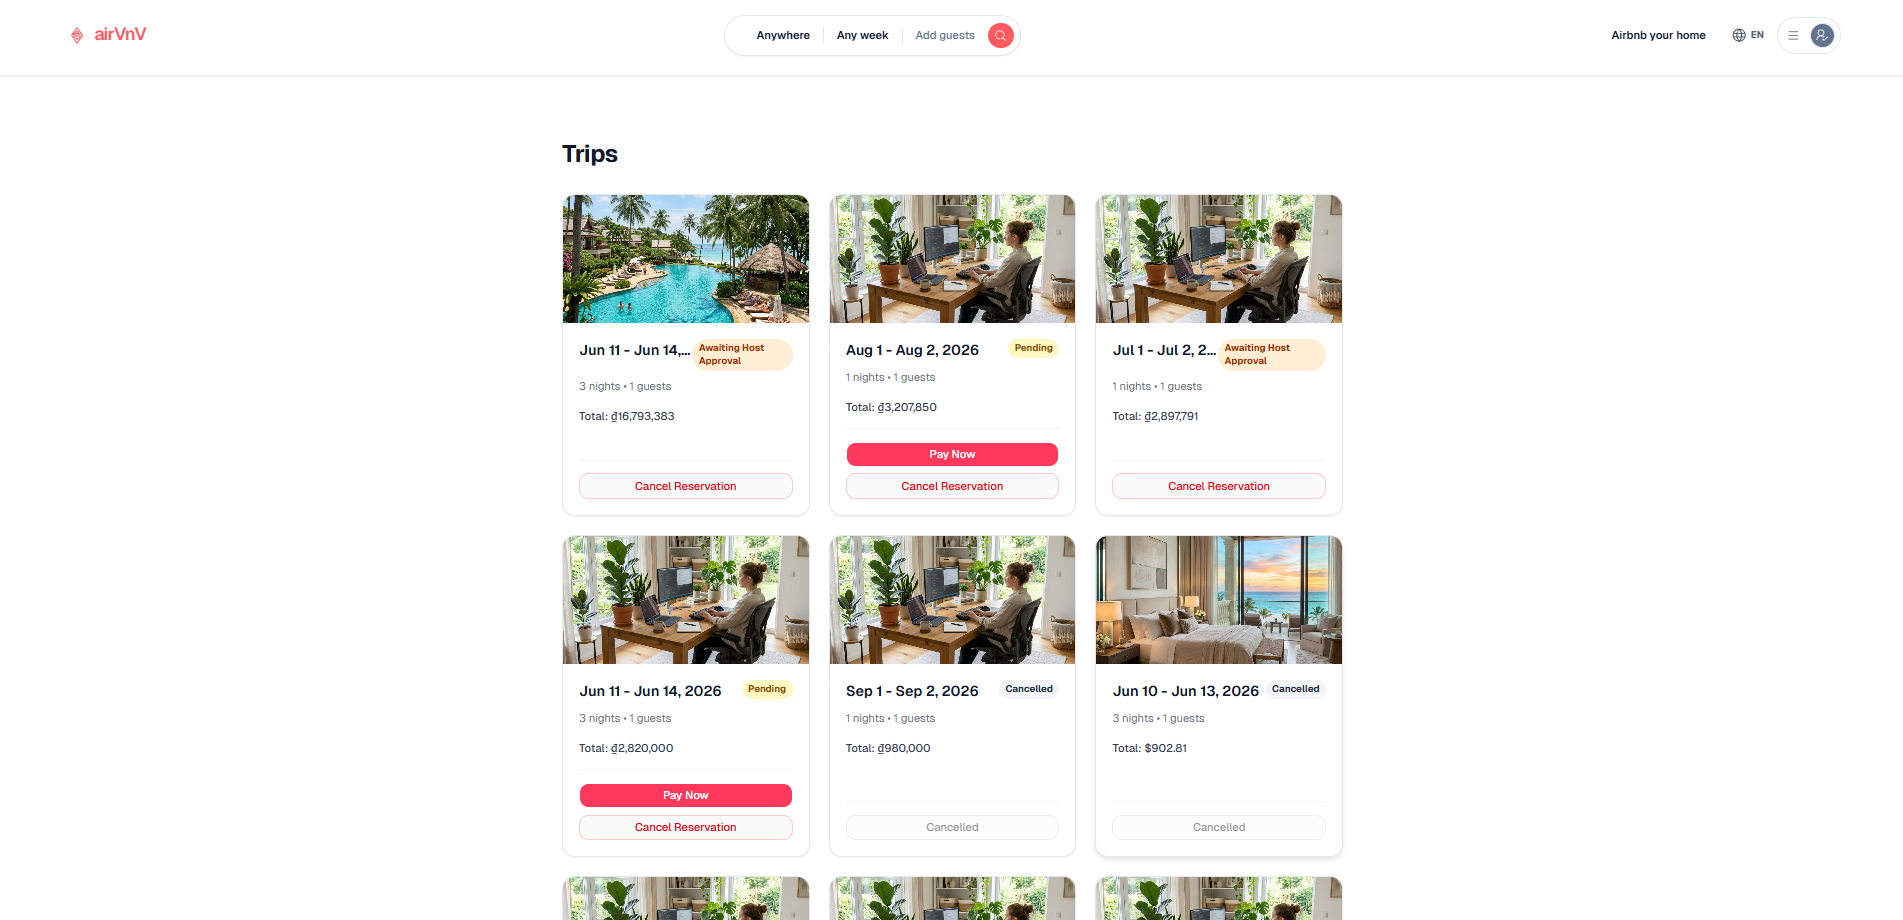
\includegraphics[width=0.85\textwidth]{figures/outputs/demo_booking.png}
  \caption{Giao diện đã Đặt phòng}
  \label{fig:demo_booking}
\end{figure}

\subsection{Thanh toán và Hoàn tiền (UC-26 -- UC-30)}
\label{subsec:tk_payment}

\texttt{PaymentService} tích hợp hai cổng thanh toán theo Strategy Pattern: \textbf{VNPay} (thanh toán trong nước) và \textbf{Stripe} (thanh toán quốc tế). \texttt{PaymentProviderResolver} đóng vai trò Factory, dựa vào cấu hình hệ thống để chọn provider phù hợp tại runtime.

Luồng thanh toán hoàn toàn bất đồng bộ:
\begin{itemize}
    \item Guest chọn phương thức thanh toán $\to$ hệ thống redirect đến VNPay/Stripe gateway.
    \item Sau khi Guest hoàn tất thanh toán trên cổng bên thứ ba, VNPay gửi \textbf{IPN (Instant Payment Notification)} callback về server.
    \item \texttt{VnpayIpn} endpoint nhận callback, xác thực chữ ký, cập nhật trạng thái Payment và phát \texttt{PaymentCompletedEvent} lên RabbitMQ.
    \item Admin có thể hoàn tiền (RefundPayment) hoặc duyệt rút tiền (ApprovePayout).
\end{itemize}

\begin{figure}[H]
  \centering
  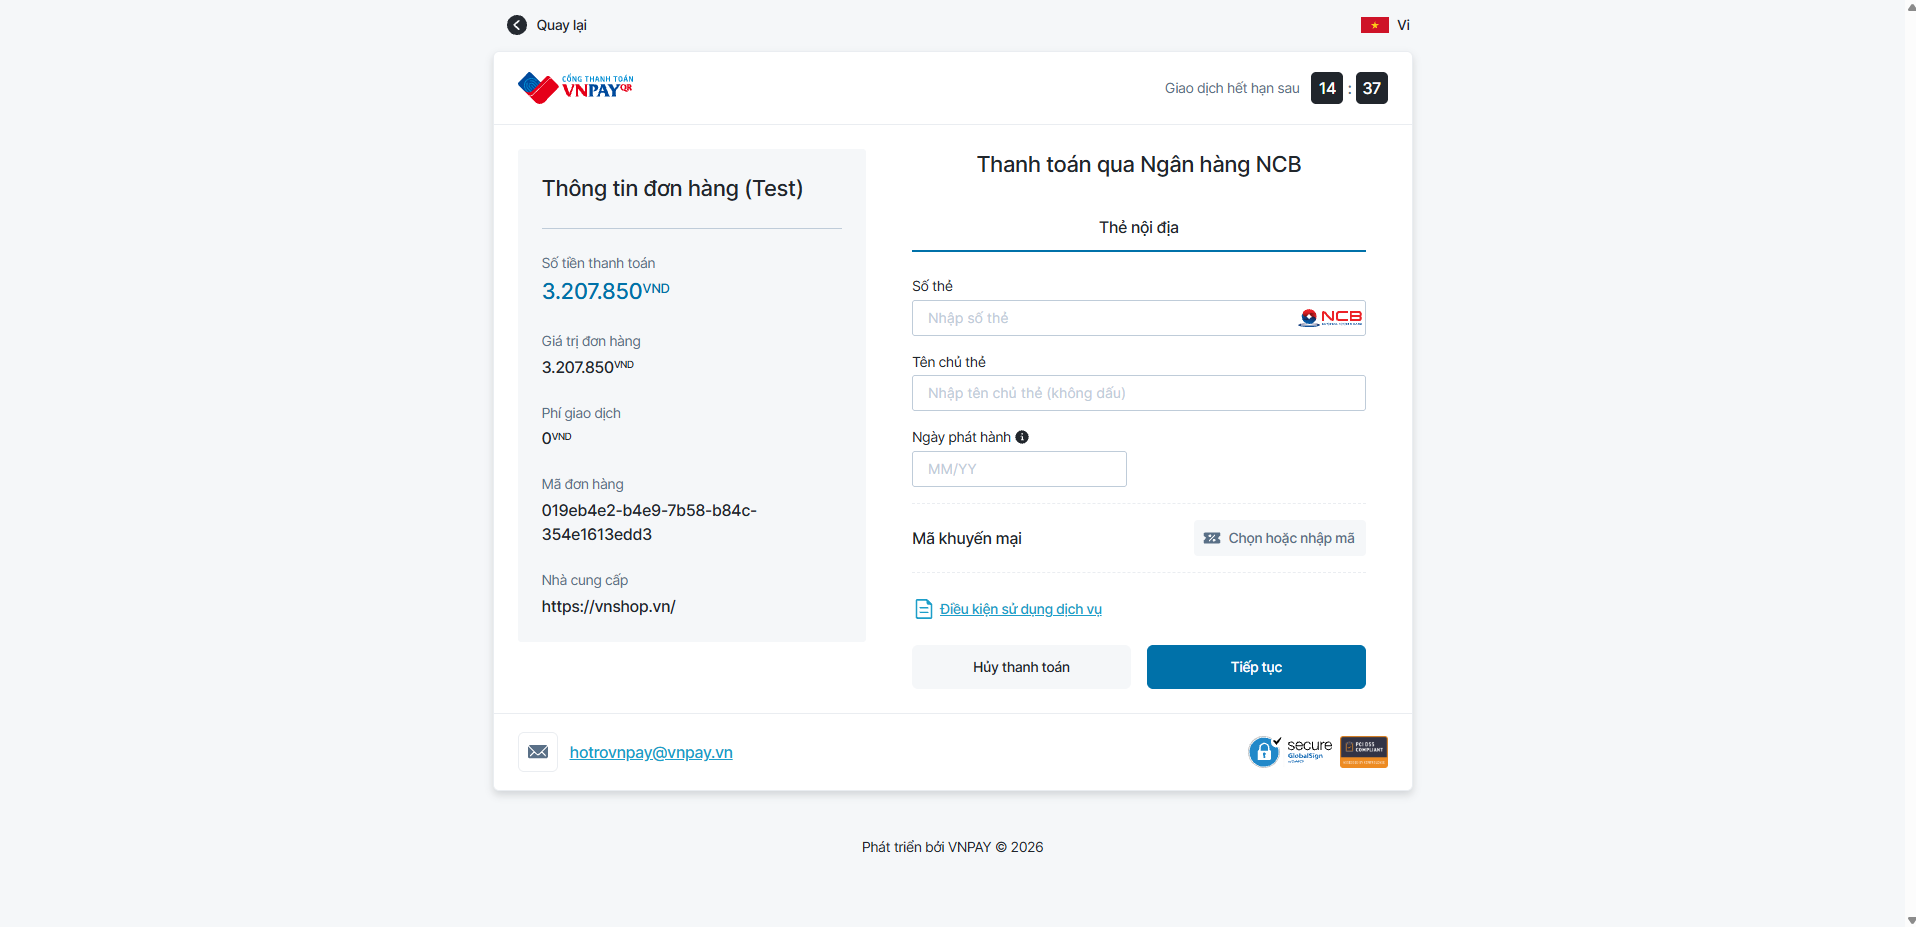
\includegraphics[width=0.85\textwidth]{figures/outputs/demo_payment.png}
  \caption{Giao diện Thanh toán VNPay}
  \label{fig:demo_payment}
\end{figure}

\subsection{Tin nhắn theo ngữ cảnh (UC-36 -- UC-40)}
\label{subsec:tk_chat}

\texttt{ChatService} triển khai hệ thống nhắn tin gắn với ngữ cảnh nghiệp vụ (property hoặc booking cụ thể). Các đặc điểm chính:

\begin{itemize}
    \item Hệ thống tự động tạo hội thoại và chèn tin nhắn hệ thống khi có sự kiện nghiệp vụ (ví dụ: \texttt{BookingConfirmedEvent} kích hoạt tin nhắn ``Đặt phòng đã được xác nhận'').
    \item Real-time qua SignalR với Redis backplane; tin nhắn được gửi tới mọi client đang kết nối với độ trễ thấp.
    \item Hỗ trợ đính kèm hình ảnh và tệp tin (GetAttachments).
    \item Đánh dấu đã đọc (MarkAsRead) và lưu trữ hội thoại (Archive).
\end{itemize}

\begin{figure}[H]
  \centering
  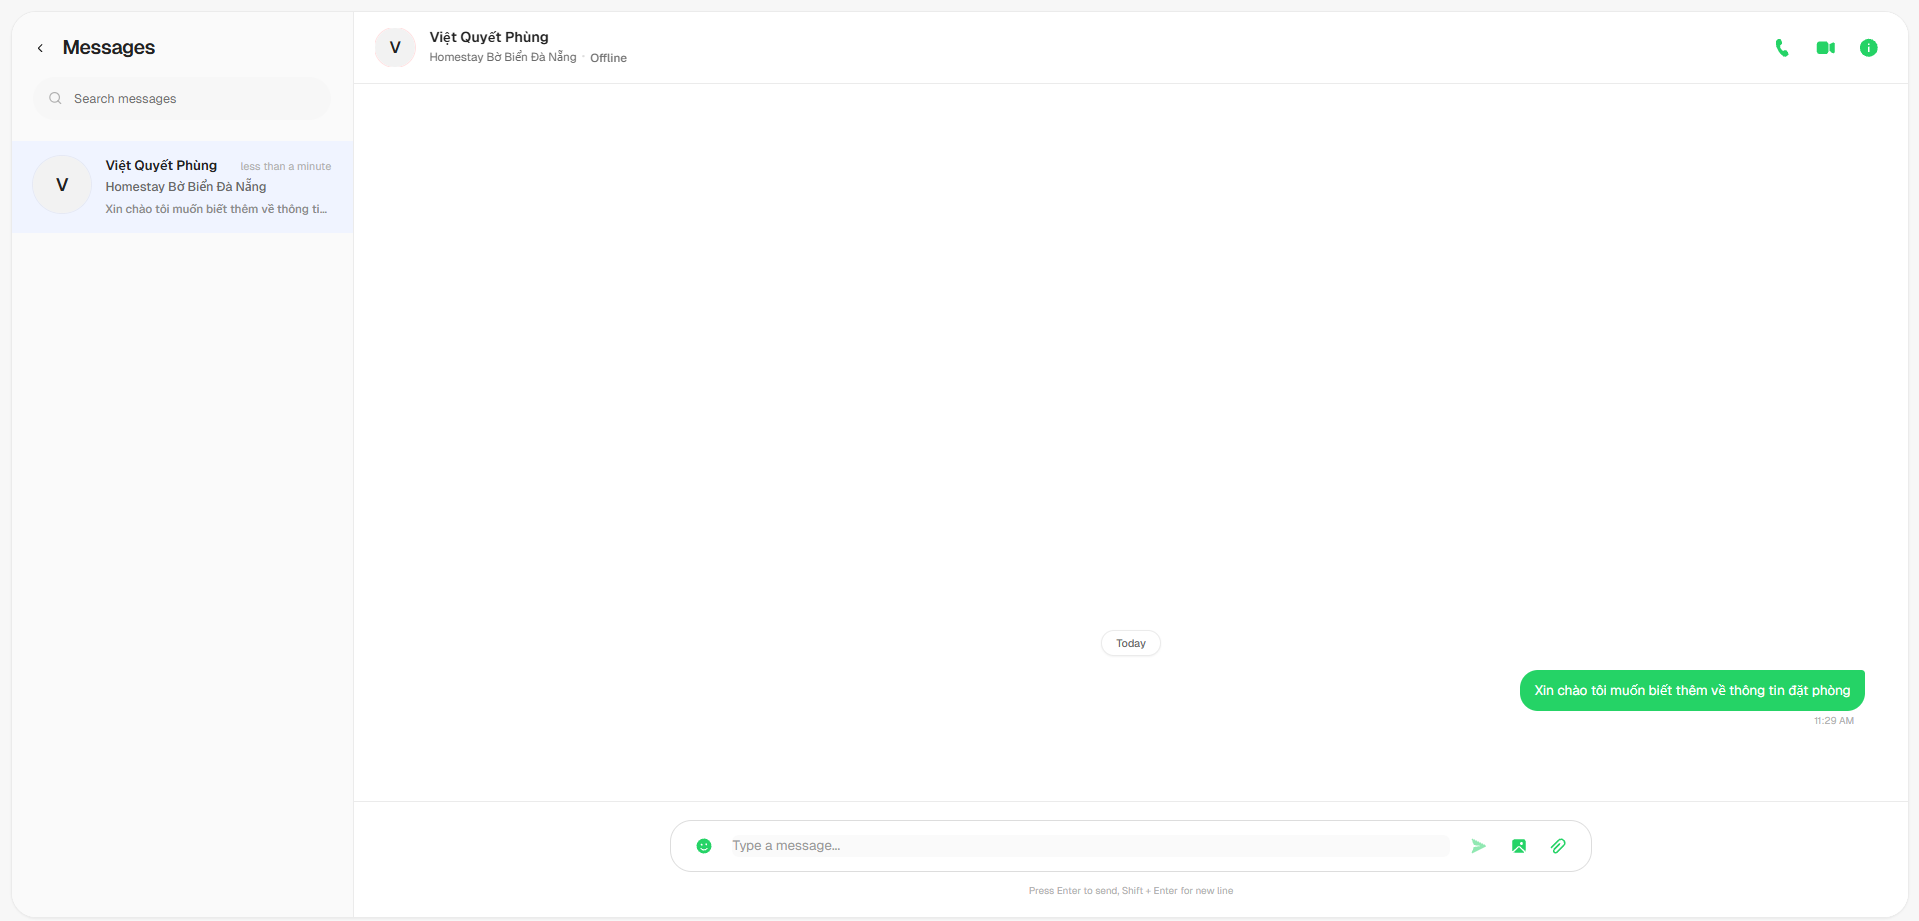
\includegraphics[width=0.85\textwidth]{figures/outputs/demo_chat.png}
  \caption{Giao diện Tin nhắn theo ngữ cảnh (Chat)}
  \label{fig:demo_chat}
\end{figure}

\subsection{Quản trị hệ thống (UC-41 -- UC-45)}
\label{subsec:tk_admin}

Giao diện Admin được xây dựng bằng Next.js 16 (App Router), cung cấp các chức năng quản trị gồm: duyệt tin đăng, quản lý người dùng, theo dõi doanh thu, xử lý thanh toán và báo cáo thống kê.

\begin{itemize}
    \item \textbf{Dashboard:} Tổng quan thống kê (số lượng Property, Booking, User, doanh thu).
    \item \textbf{Quản lý bất động sản:} Duyệt/từ chối/tạm đình chỉ tin đăng, xem chi tiết và báo cáo (phân bố giá, phân bố loại nhà, phễu trạng thái).
    \item \textbf{Quản lý người dùng:} Kích hoạt, đình chỉ, cấm người dùng. Xem báo cáo tăng trưởng.
    \item \textbf{Quản lý thanh toán:} Xem danh sách payment/payout, duyệt rút tiền, hoàn tiền, cấu hình phí nền tảng.
    \item \textbf{Báo cáo thống kê:} Biểu đồ doanh thu (Recharts), báo cáo doanh thu theo chuỗi thời gian.
\end{itemize}

\begin{figure}[H]
  \centering
  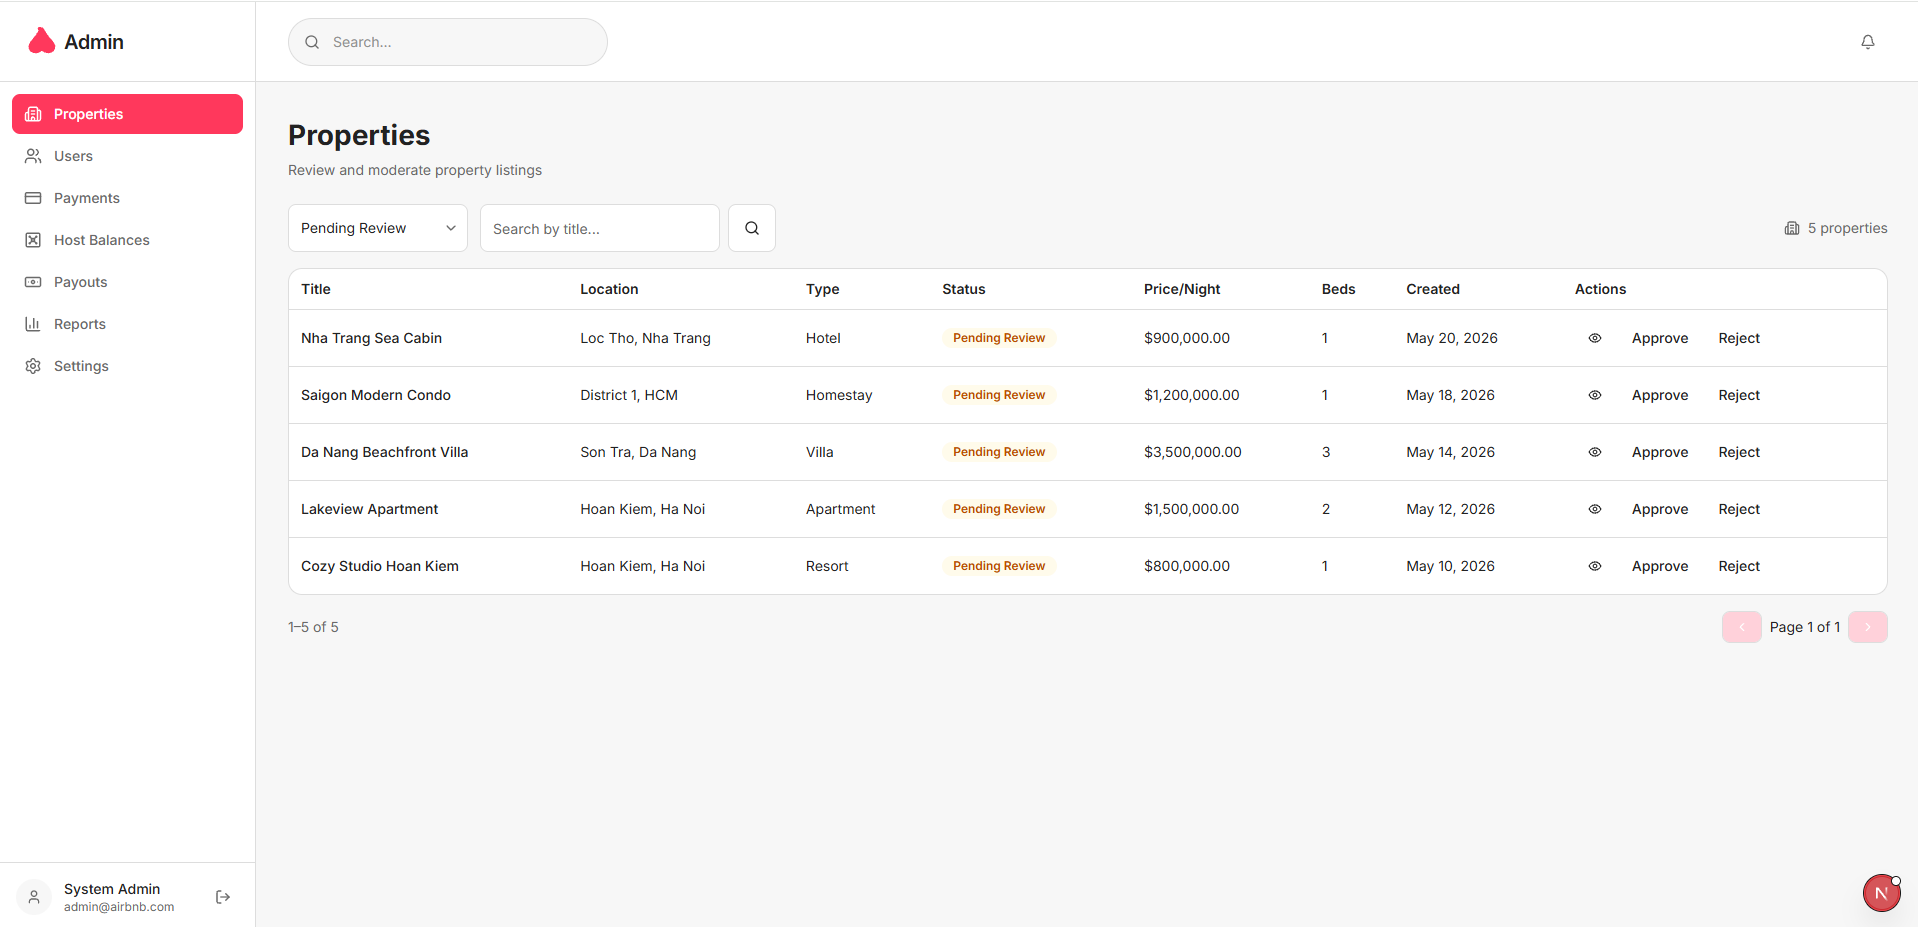
\includegraphics[width=0.85\textwidth]{figures/outputs/demo_admin_dashboard.png}
  \caption{Giao diện Dashboard Admin}
  \label{fig:demo_admin_dashboard}
\end{figure}


% -----------------------------------------------------------
\section{Đánh giá kết quả thực nghiệm}
\label{sec:danh_gia_thuc_nghiem}

\subsection{Mức độ hoàn thành Use Case}
\label{subsec:muc_do_hoan_thanh}

Đối chiếu với 45 Use Case đã được đặc tả ở Chương II, phần lớn các Use Case đã được triển khai hoàn chỉnh.

\begin{itemize}
    \item \textbf{Hoàn thành -- 44/45 (97{,}8\%):} Các chức năng thuộc bảy nhóm nghiệp vụ chính -- \textit{Xác thực và quản lý tài khoản}, \textit{Quản lý bất động sản}, \textit{Tìm kiếm}, \textit{Đặt phòng}, \textit{Đánh giá}, \textit{Tin nhắn theo ngữ cảnh} và \textit{Quản trị hệ thống} -- đã được thực hiện và chạy thử trên giao diện người dùng (xem các Hình~\ref{fig:demo_register}--\ref{fig:demo_admin_dashboard}).

    \item \textbf{Chưa triển khai -- 1/45 (2{,}2\%):} Module Xử lý khiếu nại (\textit{Disputes}) được lùi sang giai đoạn phát triển kế tiếp do phụ thuộc vào quy trình nghiệp vụ vận hành chưa được thống nhất.
\end{itemize}

Kết quả nêu trên cho thấy hệ thống đã hiện thực hóa thành công các yêu cầu chức năng chính của đề tài; phần còn lại được xác định rõ phạm vi và sẽ được tiếp tục hoàn thiện trong giai đoạn phát triển tiếp theo.

\subsection{Đánh giá hiệu năng}
\label{subsec:danh_gia_hieu_nang}

Hệ thống được đo hiệu năng trong môi trường phát triển (localhost, Docker Desktop) với bộ dữ liệu 100 bất động sản, sử dụng công cụ \textbf{k6} (Grafana). Bảng~\ref{tab:perf} trình bày kết quả đo các API nghiệp vụ chính.

\begin{table}[H]
\centering
\caption{Kết quả đo hiệu năng các API chính}
\label{tab:perf}
\renewcommand{\arraystretch}{1.3}
\begin{tabularx}{\textwidth}{|l|X|X|}
\hline
\textbf{API Endpoint} & \textbf{Response Time p95 (ms)} & \textbf{Ghi chú} \\
\hline
\texttt{POST /auth/login} & 85 & Bao gồm BCrypt hash verify \\
\hline
\texttt{GET /properties/search} & 42 & Đọc từ Elasticsearch, không chạm DB \\
\hline
\texttt{GET /properties/\{id\}} & 38 & Đọc từ PostgreSQL + cache \\
\hline
\texttt{POST /bookings} & 120 & Bao gồm kiểm tra trùng ngày + Outbox write \\
\hline
\texttt{POST /payments/initiate} & 95 & Tạo Payment record + redirect URL \\
\hline
\texttt{POST /chat/conversations} & 60 & Kiểm tra quyền + tạo conversation \\
\hline
\texttt{GET /chat/messages} & 35 & Phân trang, đọc từ PostgreSQL \\
\hline
\end{tabularx}
\end{table}

\noindent Kết quả cho thấy:
\begin{itemize}
    \item Tất cả API đáp ứng yêu cầu phi chức năng \textbf{response time $\leq$ 500ms (p95)} (Bảng~\ref{tab:nfr}, Chương II).
    \item API tìm kiếm đạt \textbf{42ms (p95)}, thấp hơn đáng kể so với mục tiêu $\leq$ 200ms nhờ kiến trúc CQRS với Elasticsearch read-model.
    \item API đặt phòng có response time cao nhất (120ms) do cần kiểm tra trùng ngày và ghi Outbox message trong cùng transaction, nhưng vẫn nằm trong ngưỡng cho phép.
\end{itemize}

\subsection{Đánh giá tính nhất quán dữ liệu}
\label{subsec:danh_gia_nhat_quan}

\subsubsection{Transactional Outbox Pattern}
\label{subsubsec:danh_gia_outbox}

Để kiểm chứng Outbox Pattern hoạt động đúng, nhóm thực hiện bài test: tạo Booking đồng thời tắt RabbitMQ. Kết quả:
\begin{itemize}
    \item Event \texttt{BookingCreatedEvent} được ghi vào bảng \texttt{OutboxMessage} trong cùng transaction với Booking record.
    \item Sau khi RabbitMQ khởi động lại, MassTransit background worker tự động quét bảng Outbox và publish event đang chờ.
    \item \texttt{PaymentService} nhận event và xử lý bình thường $\to$ không mất sự kiện nghiệp vụ.
\end{itemize}

\subsubsection{Đồng bộ CDC (Debezium $\to$ Kafka $\to$ Elasticsearch)}
\label{subsubsec:danh_gia_cdc}

Nhóm thực hiện kiểm tra đồng bộ dữ liệu bằng cách:
\begin{enumerate}
    \item Tạo Property mới qua \texttt{PropertyService} (ghi vào PostgreSQL).
    \item Quan sát Debezium bắt thay đổi từ WAL log và publish vào Kafka topic.
    \item \texttt{SearchService} tiêu thụ event và index vào Elasticsearch.
    \item Gọi API tìm kiếm $\to$ Property mới xuất hiện trong kết quả.
\end{enumerate}

Độ trễ đồng bộ (CDC latency) đo được trung bình $\approx$ 1--3 giây từ lúc ghi PostgreSQL đến khi xuất hiện trên Elasticsearch, đáp ứng yêu cầu eventual consistency.

\subsection{Đánh giá bảo mật cơ bản}
\label{subsec:danh_gia_bao_mat}

\begin{itemize}
    \item \textbf{Xác thực JWT:} YARP API Gateway validate JWT trên mọi endpoint bảo vệ. Request không có token hoặc token hết hạn trả về \texttt{401 Unauthorized}.
    \item \textbf{Phân quyền theo Role:} Endpoints Admin yêu cầu role \texttt{Admin} hoặc \texttt{Moderator}; endpoints Host yêu cầu role \texttt{Host}; trả về \texttt{403 Forbidden} nếu không đủ quyền.
    \item \textbf{Mã hóa mật khẩu:} BCrypt với work factor mặc định, không lưu plaintext.
    \item \textbf{Chống double-booking:} Unique filtered index ở tầng PostgreSQL đảm bảo một phòng không bị đặt trùng hai lần cùng ngày, kể cả khi có race condition.
\end{itemize}
